\chapter[Multicolinearidade]{Multicolinearidade em Modelagem de Distribuição de Espécies}

\begin{objetivos}
	Ao final desta unidade, o estudante deverá ser capaz de compreender o conceito de multicolinearidade em SDM; identificar variáveis ambientais redundantes por correlação; calcular e interpretar o Fator de Inflação da Variância (VIF); compreender os efeitos da colinearidade sobre interpretação ecológica, estabilidade dos parâmetros e transferibilidade dos modelos; aplicar PCA como estratégia de redução dimensional; e construir um fluxo reprodutível em R para seleção e transformação de variáveis ambientais antes da modelagem.
\end{objetivos}

\section{Introdução}

A multicolinearidade ocorre quando duas ou mais variáveis preditoras carregam informação semelhante. Em Modelagem de Distribuição de Espécies, esse problema é comum porque variáveis climáticas, topográficas, edáficas e hidrológicas frequentemente covariam no espaço. Por exemplo, temperatura média anual pode estar fortemente associada à altitude; precipitação anual pode estar correlacionada com precipitação do trimestre mais úmido; e variáveis topográficas derivadas de um mesmo modelo digital de elevação podem apresentar forte redundância.

A presença de variáveis altamente correlacionadas pode gerar modelos instáveis, dificultar a interpretação da importância das variáveis, inflar incertezas em modelos paramétricos e reduzir a capacidade de transferência espacial ou temporal. Por isso, a seleção de preditores ambientais deve combinar fundamentação ecológica, análise exploratória e critérios estatísticos \parencite{guisan2017habitat,naimi2016sdm,raes2018modeling}.

\begin{atencao}[title={\faExclamationTriangle\quad Mais variáveis não significam melhor modelo}]
	Adicionar muitas variáveis ambientais não garante melhor desempenho. Variáveis redundantes podem aumentar complexidade, gerar instabilidade, dificultar interpretação ecológica e reduzir a transferibilidade do modelo.
\end{atencao}

\section{O problema da multicolinearidade}

Variáveis ambientais frequentemente apresentam forte correlação entre si. Em regiões tropicais, por exemplo, áreas com elevada precipitação anual frequentemente apresentam baixa sazonalidade hídrica, enquanto gradientes térmicos podem estar associados a gradientes altitudinais.

Quando duas ou mais variáveis carregam informação semelhante, ocorre multicolinearidade. Embora a capacidade preditiva do modelo possa permanecer elevada, a interpretação ecológica dos coeficientes torna-se instável e a transferência espacial ou temporal pode ser comprometida \parencite{dormann2013collinearity}.

\section{Correlação entre variáveis ambientais}

A forma mais simples de diagnosticar redundância entre preditores é calcular correlações par a par. Em SDM, os coeficientes de Pearson e Spearman são os mais utilizados. Pearson mede associação linear entre variáveis contínuas, enquanto Spearman avalia associação monotônica baseada em postos, sendo útil quando as distribuições não são normais ou apresentam assimetria.

Na prática, muitos estudos usam limiares como \(|r| > 0{,}7\) ou \(|r| > 0{,}8\) para indicar alta correlação. Esses limiares não devem ser tratados como regras absolutas, mas como critérios operacionais. Quando duas variáveis estão fortemente correlacionadas, recomenda-se manter aquela com maior relevância ecológica, maior qualidade espacial, maior interpretabilidade ou melhor adequação ao objetivo do estudo \parencite{dormann2013collinearity,raes2018modeling}.

\begin{conceito}[title={\faBook\quad Correlação não é causalidade}]
	Duas variáveis podem ser altamente correlacionadas sem que uma cause a outra. Em SDM, a correlação indica redundância informacional, mas a decisão sobre qual variável manter deve considerar a ecologia da espécie e a hipótese do estudo.
\end{conceito}

\begin{conceito}[title={\faBook\quad Correlação não implica redundância ecológica}]
	Duas variáveis podem apresentar alta correlação estatística e, ainda assim, representar processos ecológicos distintos.
	
	Por exemplo, precipitação anual e precipitação do trimestre mais seco podem ser altamente correlacionadas, mas representam mecanismos ecológicos diferentes relacionados à disponibilidade hídrica.
\end{conceito}

\rscriptfile{scripts/unidade04/01_estrutura_pastas.R}

\rscriptfile{scripts/unidade04/02_preparar_variaveis_colineares.R}

\rscriptfile{scripts/unidade04/03_correlacao_variaveis.R}

\begin{figure}[H]
	\centering
	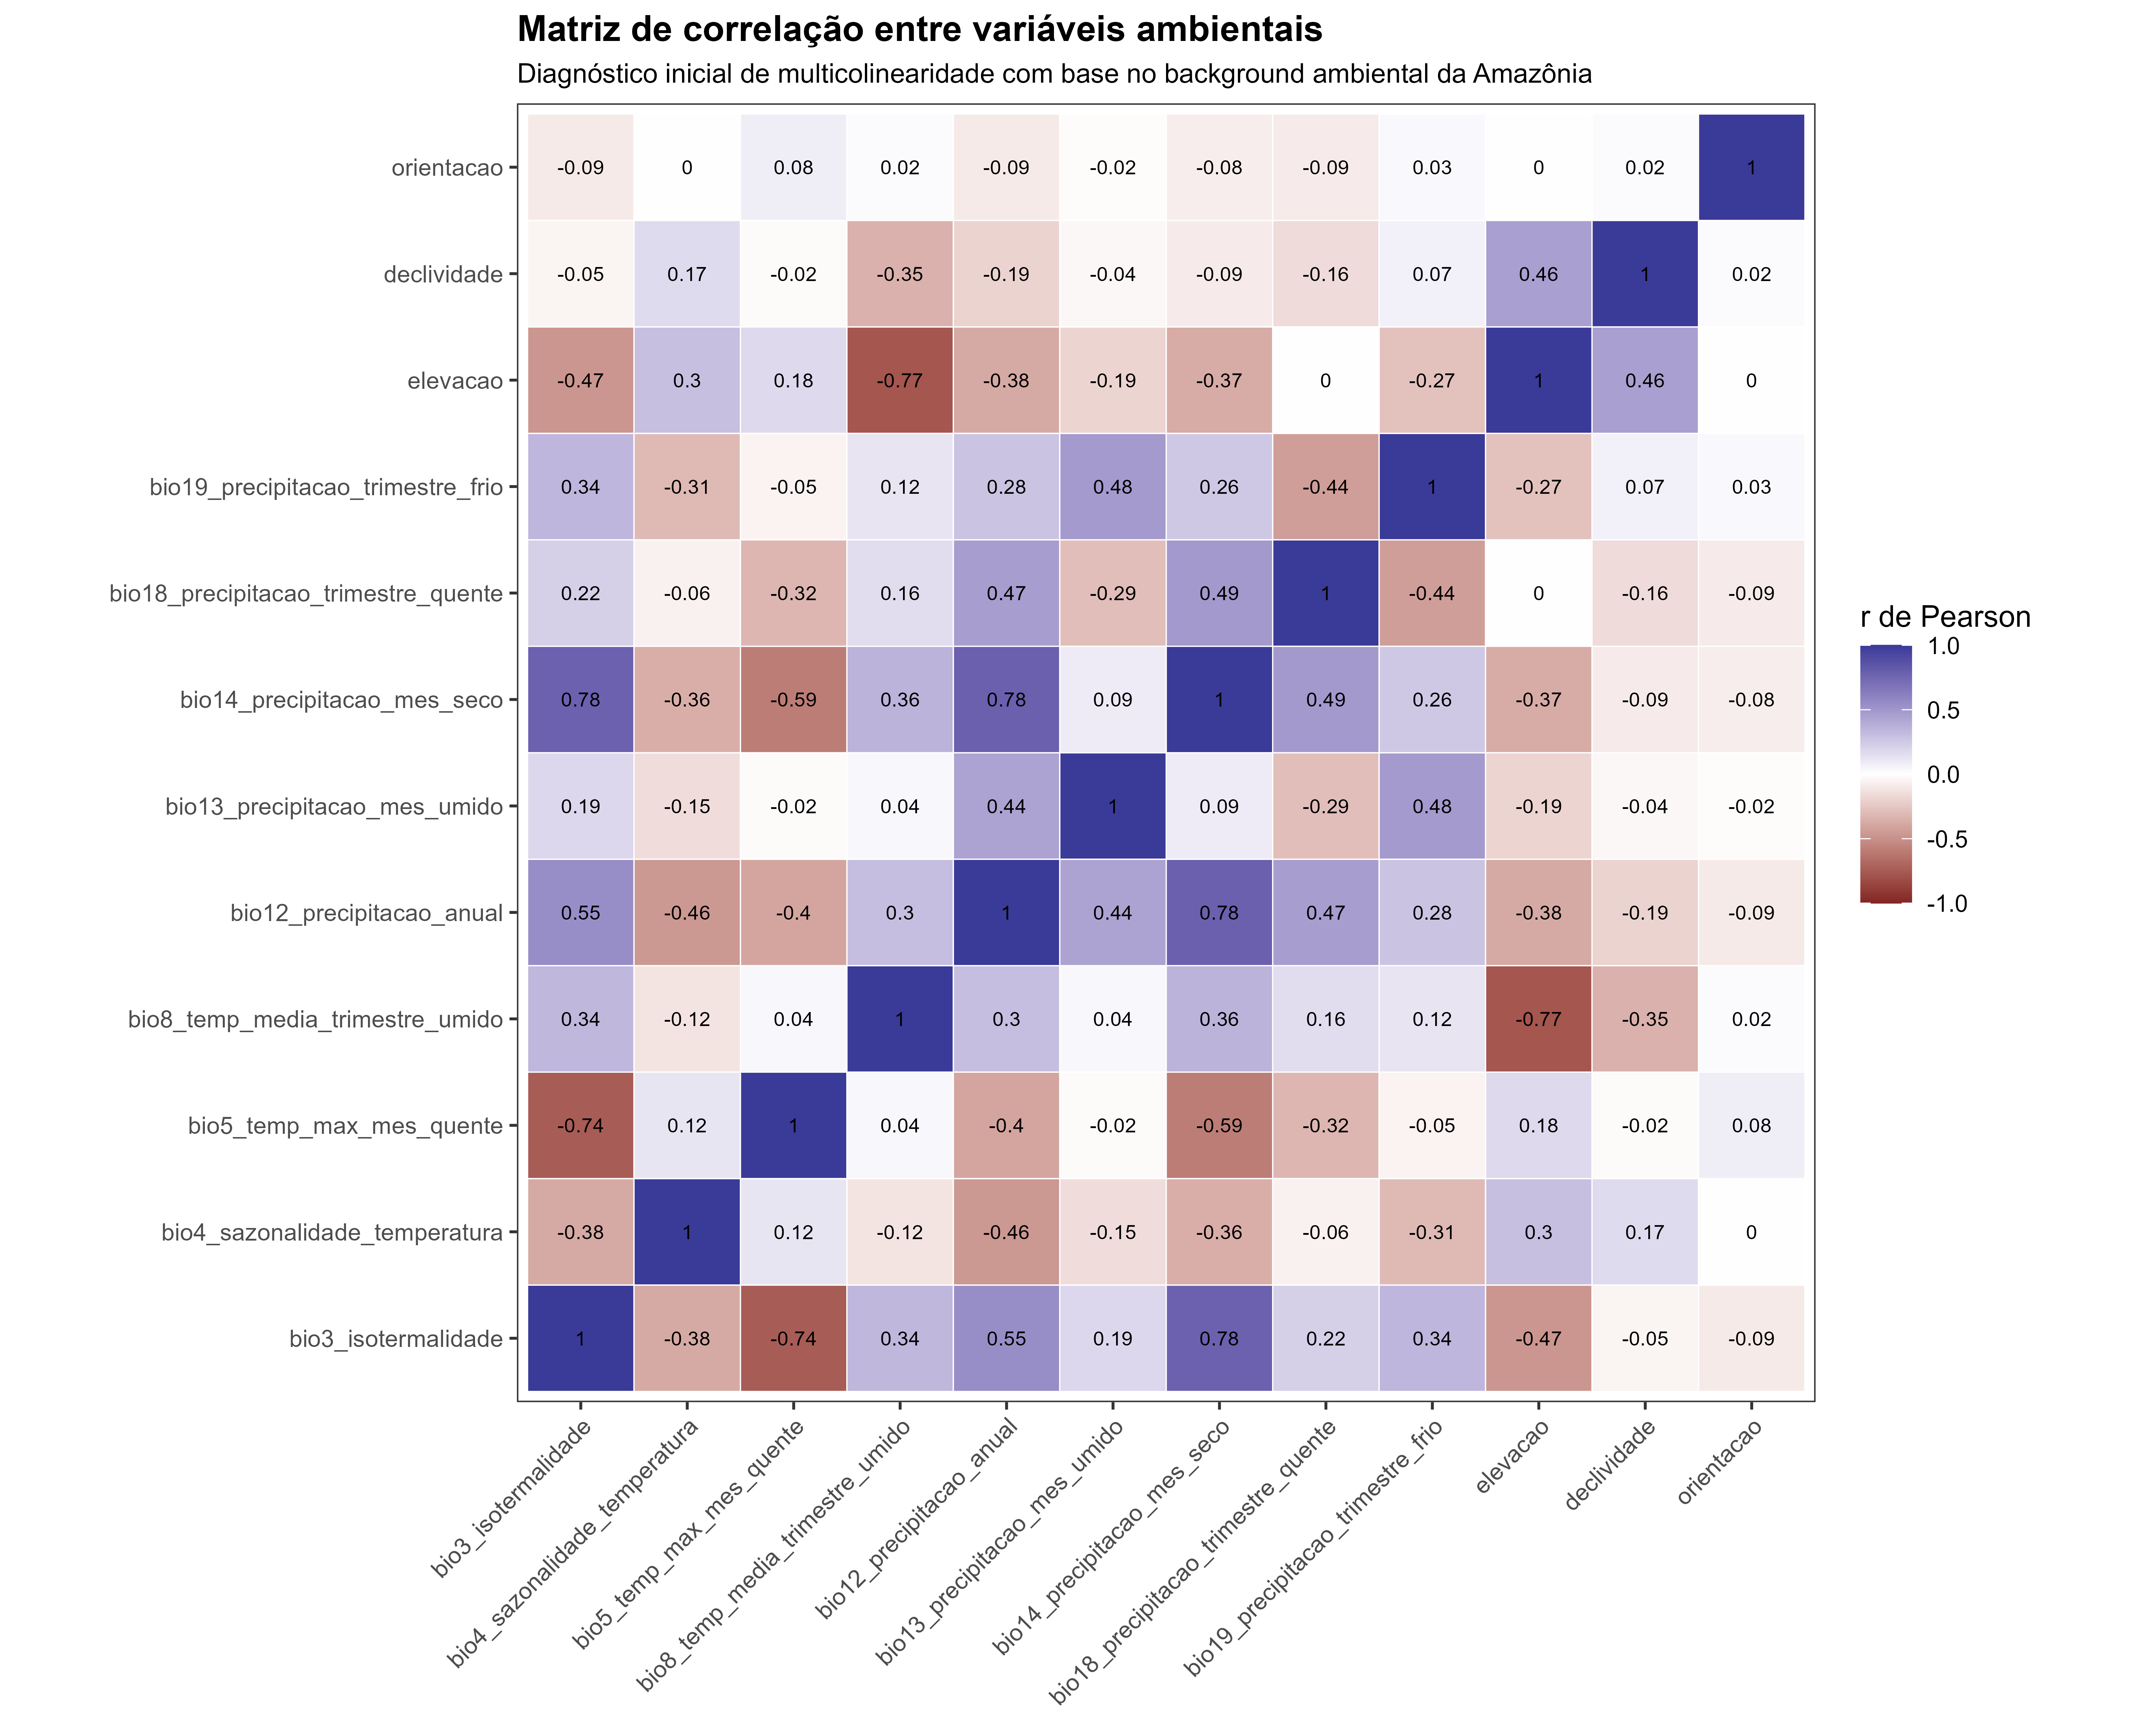
\includegraphics[width=\textwidth]
	{figuras/unidade04/unidade04_matriz_correlacao.png}
	\caption{
		Matriz de correlação de Pearson entre as variáveis ambientais
		utilizadas para modelagem de \textit{Dinizia excelsa}
		no bioma Amazônia.
		Os coeficientes indicam a intensidade da associação linear
		entre pares de variáveis ambientais.
	}
	\label{fig:unidade04_matriz_correlacao}
\end{figure}

\section{Fator de Inflação da Variância}

O Fator de Inflação da Variância, conhecido como VIF, avalia o quanto a variância estimada de um coeficiente é inflada pela dependência linear entre uma variável preditora e todas as demais. Diferentemente da correlação par a par, o VIF considera a relação de cada variável com o conjunto completo dos preditores.

\begin{equationbox}
	\[
	VIF_j = \frac{1}{1 - R_j^2}
	\]
	
	Em que \(VIF_j\) é o Fator de Inflação da Variância da variável \(j\), e \(R_j^2\) é o coeficiente de determinação obtido ao ajustar uma regressão da variável \(j\) contra todas as demais variáveis preditoras.
\end{equationbox}

Valores elevados de VIF indicam que uma variável pode ser explicada por uma combinação das outras. Como regra prática, VIF acima de 10 é frequentemente interpretado como evidência de colinearidade severa, embora limiares mais conservadores, como 5, também sejam usados em estudos ecológicos \parencite{obrien2007vif,dormann2013collinearity,naimi2016sdm}.

\begin{dica}[title={\faLightbulb\quad Correlação e VIF são complementares}]
	A correlação identifica pares de variáveis redundantes. O VIF identifica variáveis redundantes em relação ao conjunto completo de preditores. Em estudos robustos, os dois diagnósticos devem ser avaliados conjuntamente.
\end{dica}

\rscriptfile{scripts/unidade04/04_vif_variaveis.R}

\begin{figure}[H]
	\centering
	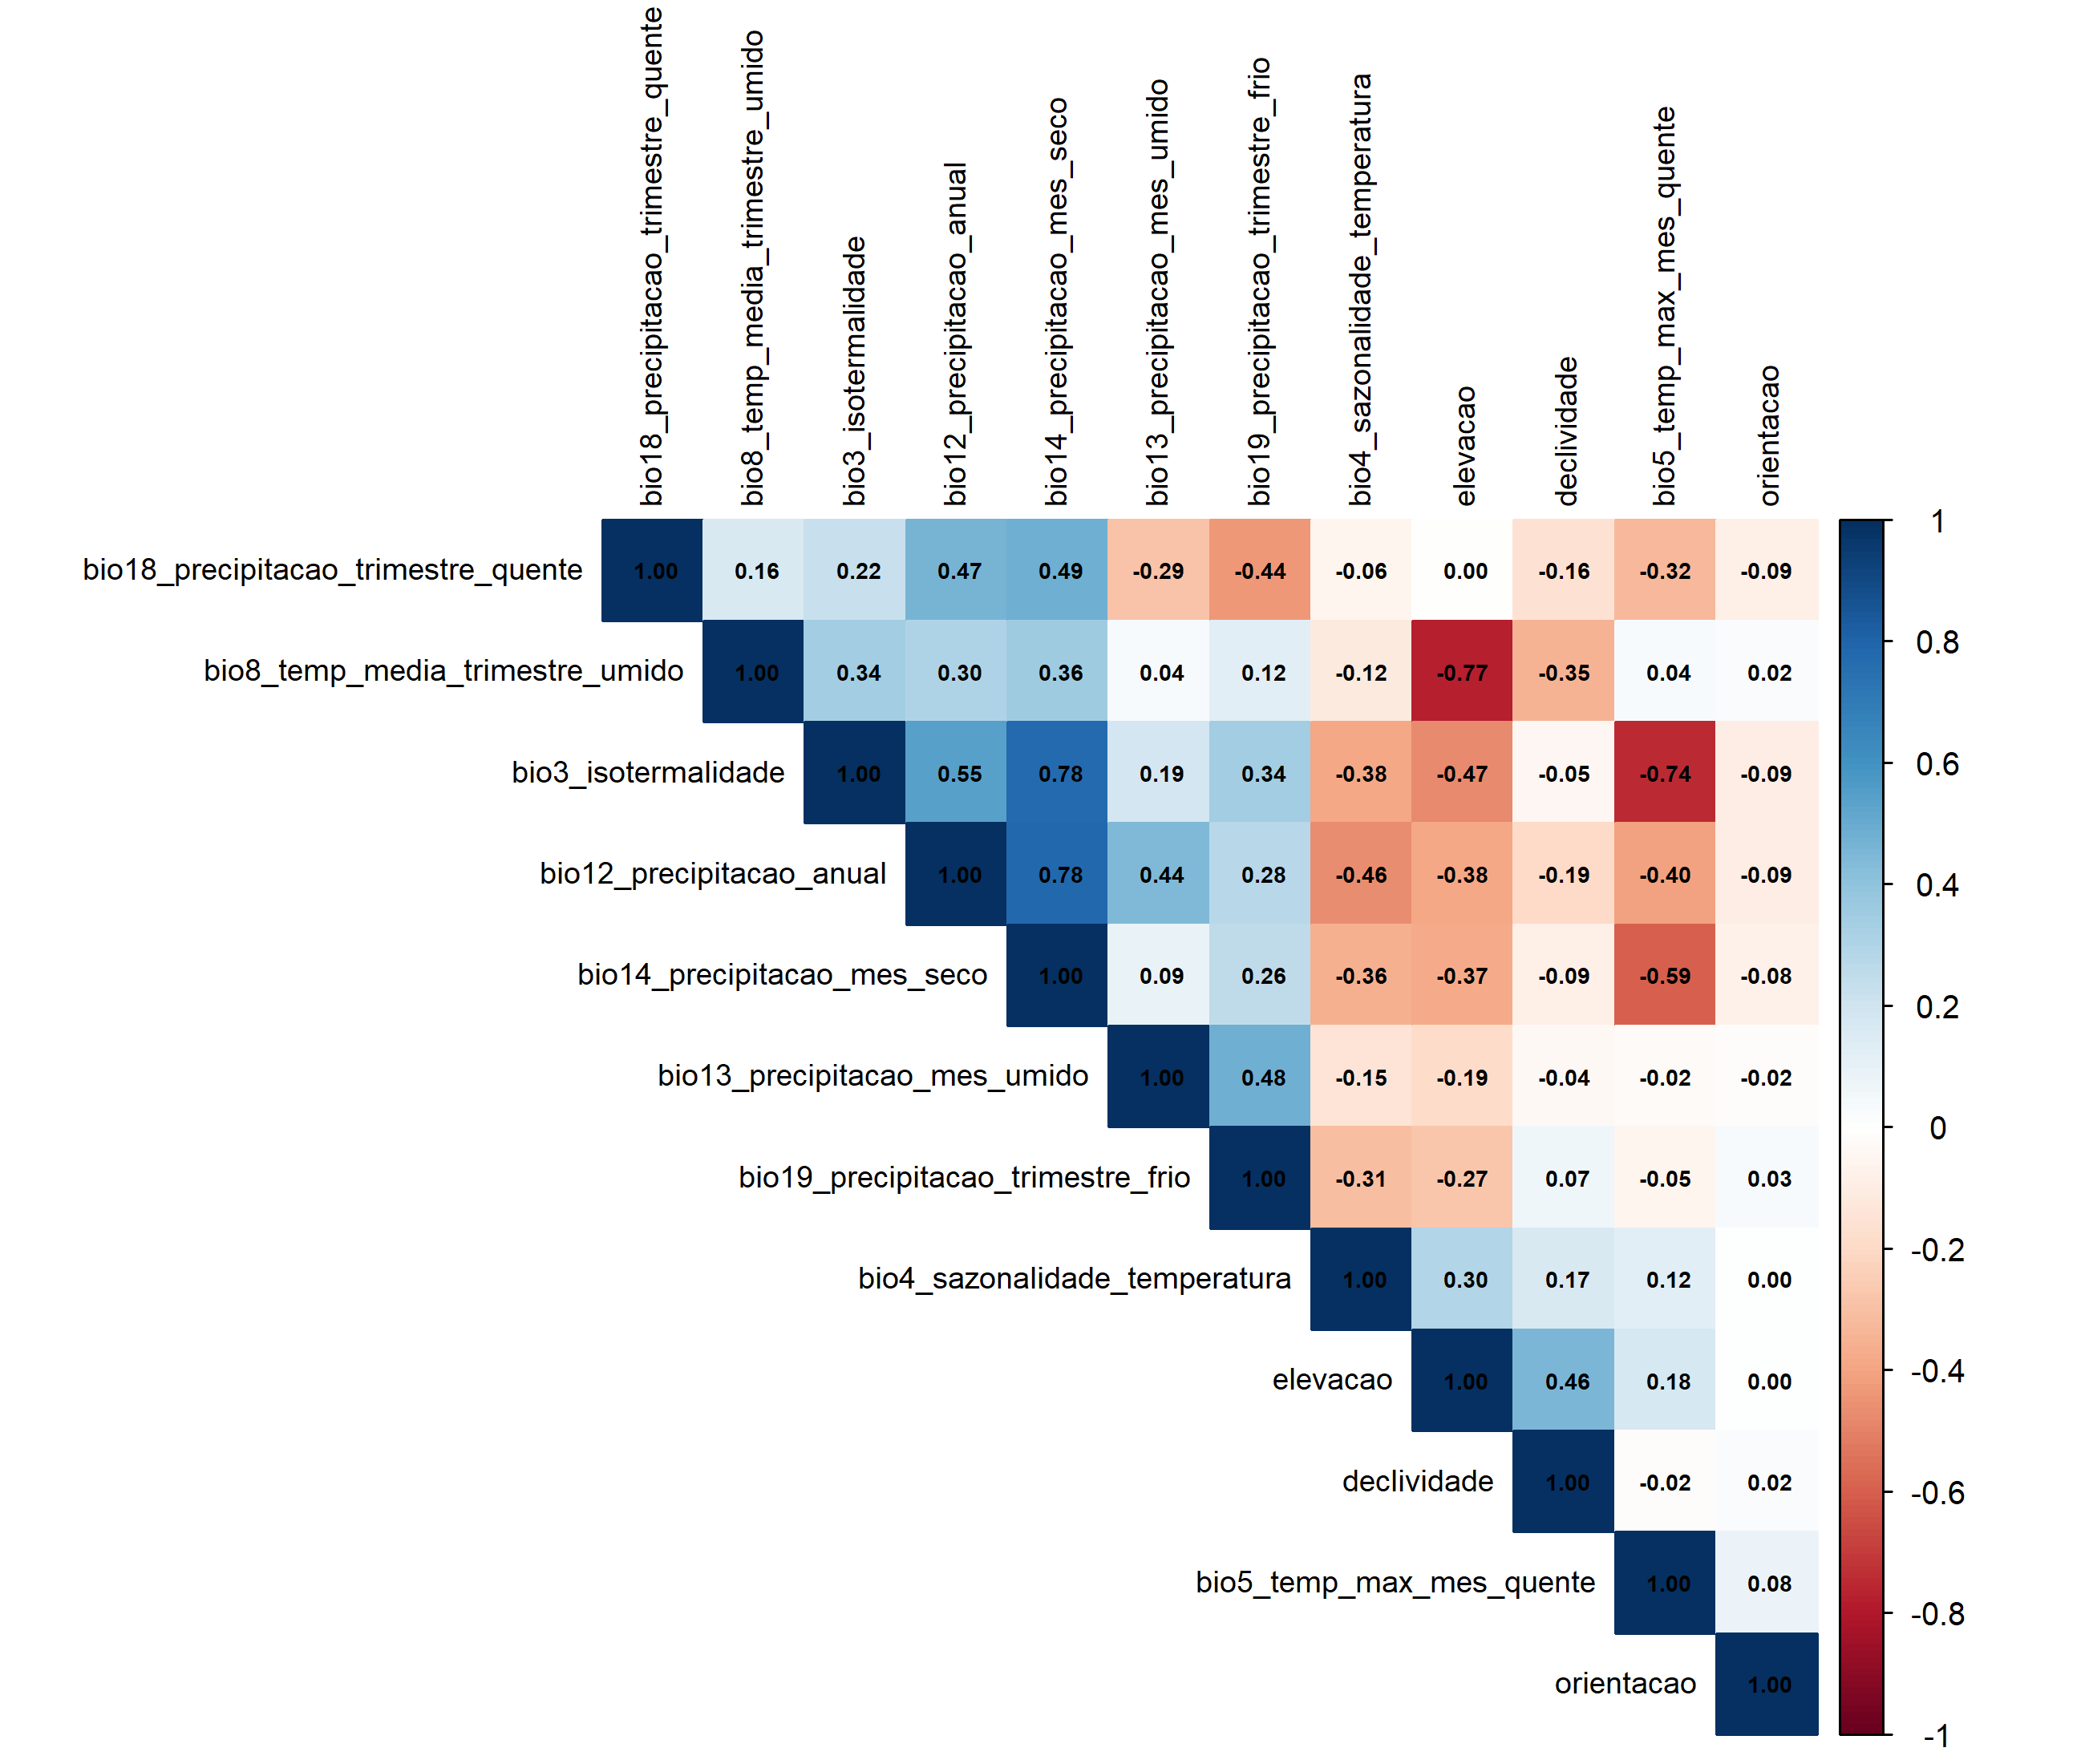
\includegraphics[width=0.95\textwidth]
	{figuras/unidade04/unidade04_corrplot_correlacao.png}
	\caption{
		Representação gráfica da correlação entre variáveis ambientais.
		Cores mais intensas representam correlações mais fortes,
		enquanto correlações próximas de zero indicam maior independência
		entre variáveis.
	}
	\label{fig:unidade04_corrplot}
\end{figure}

\begin{figure}[H]
	\centering
	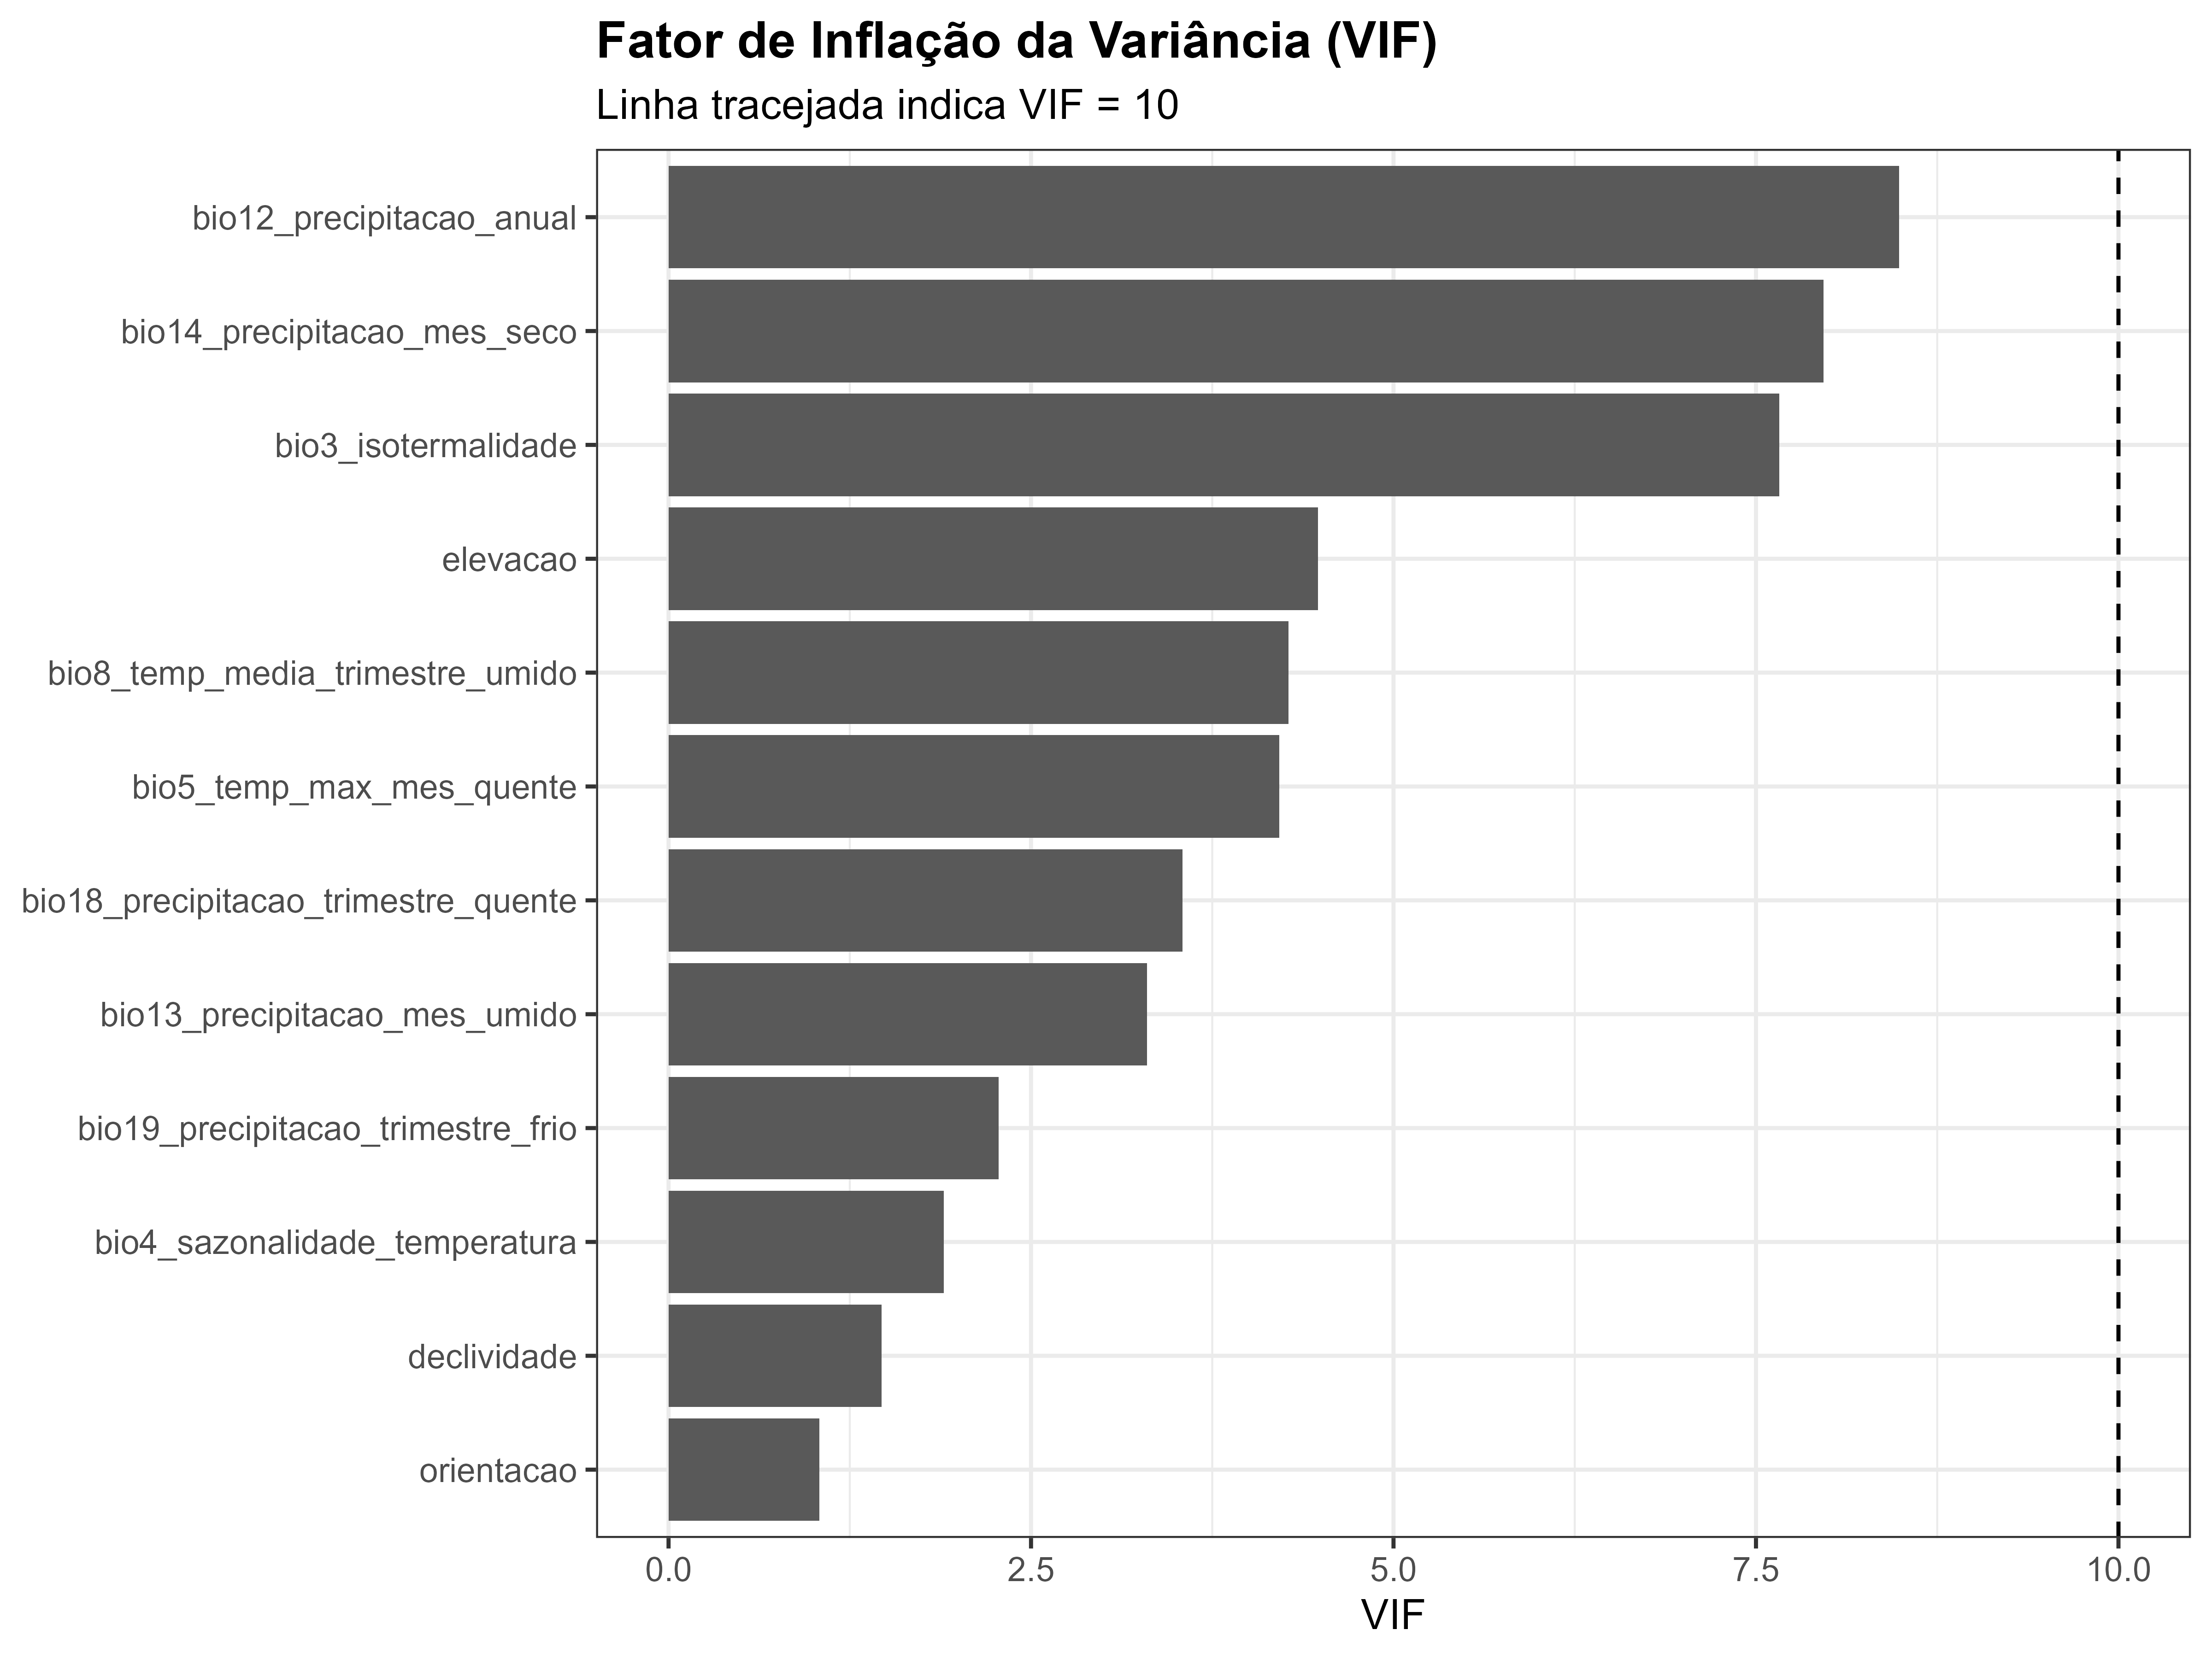
\includegraphics[width=0.85\textwidth]
	{figuras/unidade04/unidade04_vif_variaveis.png}
	\caption{
		Valores do Fator de Inflação da Variância (VIF)
		para as variáveis ambientais avaliadas.
		A linha tracejada representa o limiar adotado
		para identificação de multicolinearidade excessiva.
	}
	\label{fig:unidade04_vif}
\end{figure}

\begin{aplicacao}
	As Figuras~\ref{fig:unidade04_matriz_correlacao}
	e~\ref{fig:unidade04_corrplot}
	permitem identificar conjuntos de variáveis que carregam
	informação semelhante.
	
	Em SDM, manter simultaneamente variáveis altamente correlacionadas
	pode dificultar a interpretação ecológica dos modelos e aumentar
	a instabilidade das projeções espaciais e temporais.
\end{aplicacao}

\begin{aplicacao}
	O VIF quantifica o quanto a variância de uma variável
	é inflacionada pela presença de correlação com outras variáveis.
	
	Valores elevados indicam redundância estatística
	e sugerem que a variável deve ser removida ou substituída
	por outra ecologicamente mais representativa.
\end{aplicacao}

\section{Seleção de variáveis ambientais}

A seleção de variáveis deve equilibrar três dimensões: relevância ecológica, qualidade dos dados e redundância estatística. Remover automaticamente variáveis apenas com base em limiares pode gerar modelos pobres do ponto de vista ecológico. Por outro lado, manter variáveis redundantes pode gerar modelos difíceis de interpretar.

Em SDM, recomenda-se iniciar com um conjunto amplo de variáveis candidatas, justificar ecologicamente cada grupo de preditores e, em seguida, aplicar filtros de correlação e VIF. Quando duas variáveis são correlacionadas, a decisão deve priorizar aquela com relação mais direta com processos ecológicos, maior estabilidade temporal, melhor resolução ou menor erro conhecido.

\begin{atencao}[title={\faExclamationTriangle\quad Não selecione variáveis apenas pelo algoritmo}]
	A seleção automática pode remover variáveis ecologicamente importantes e manter variáveis estatisticamente convenientes, mas biologicamente frágeis. A seleção de preditores deve ser documentada e justificada.
\end{atencao}

\rscriptfile{scripts/unidade04/05_selecao_variaveis.R}

\begin{figure}[H]
	\centering
	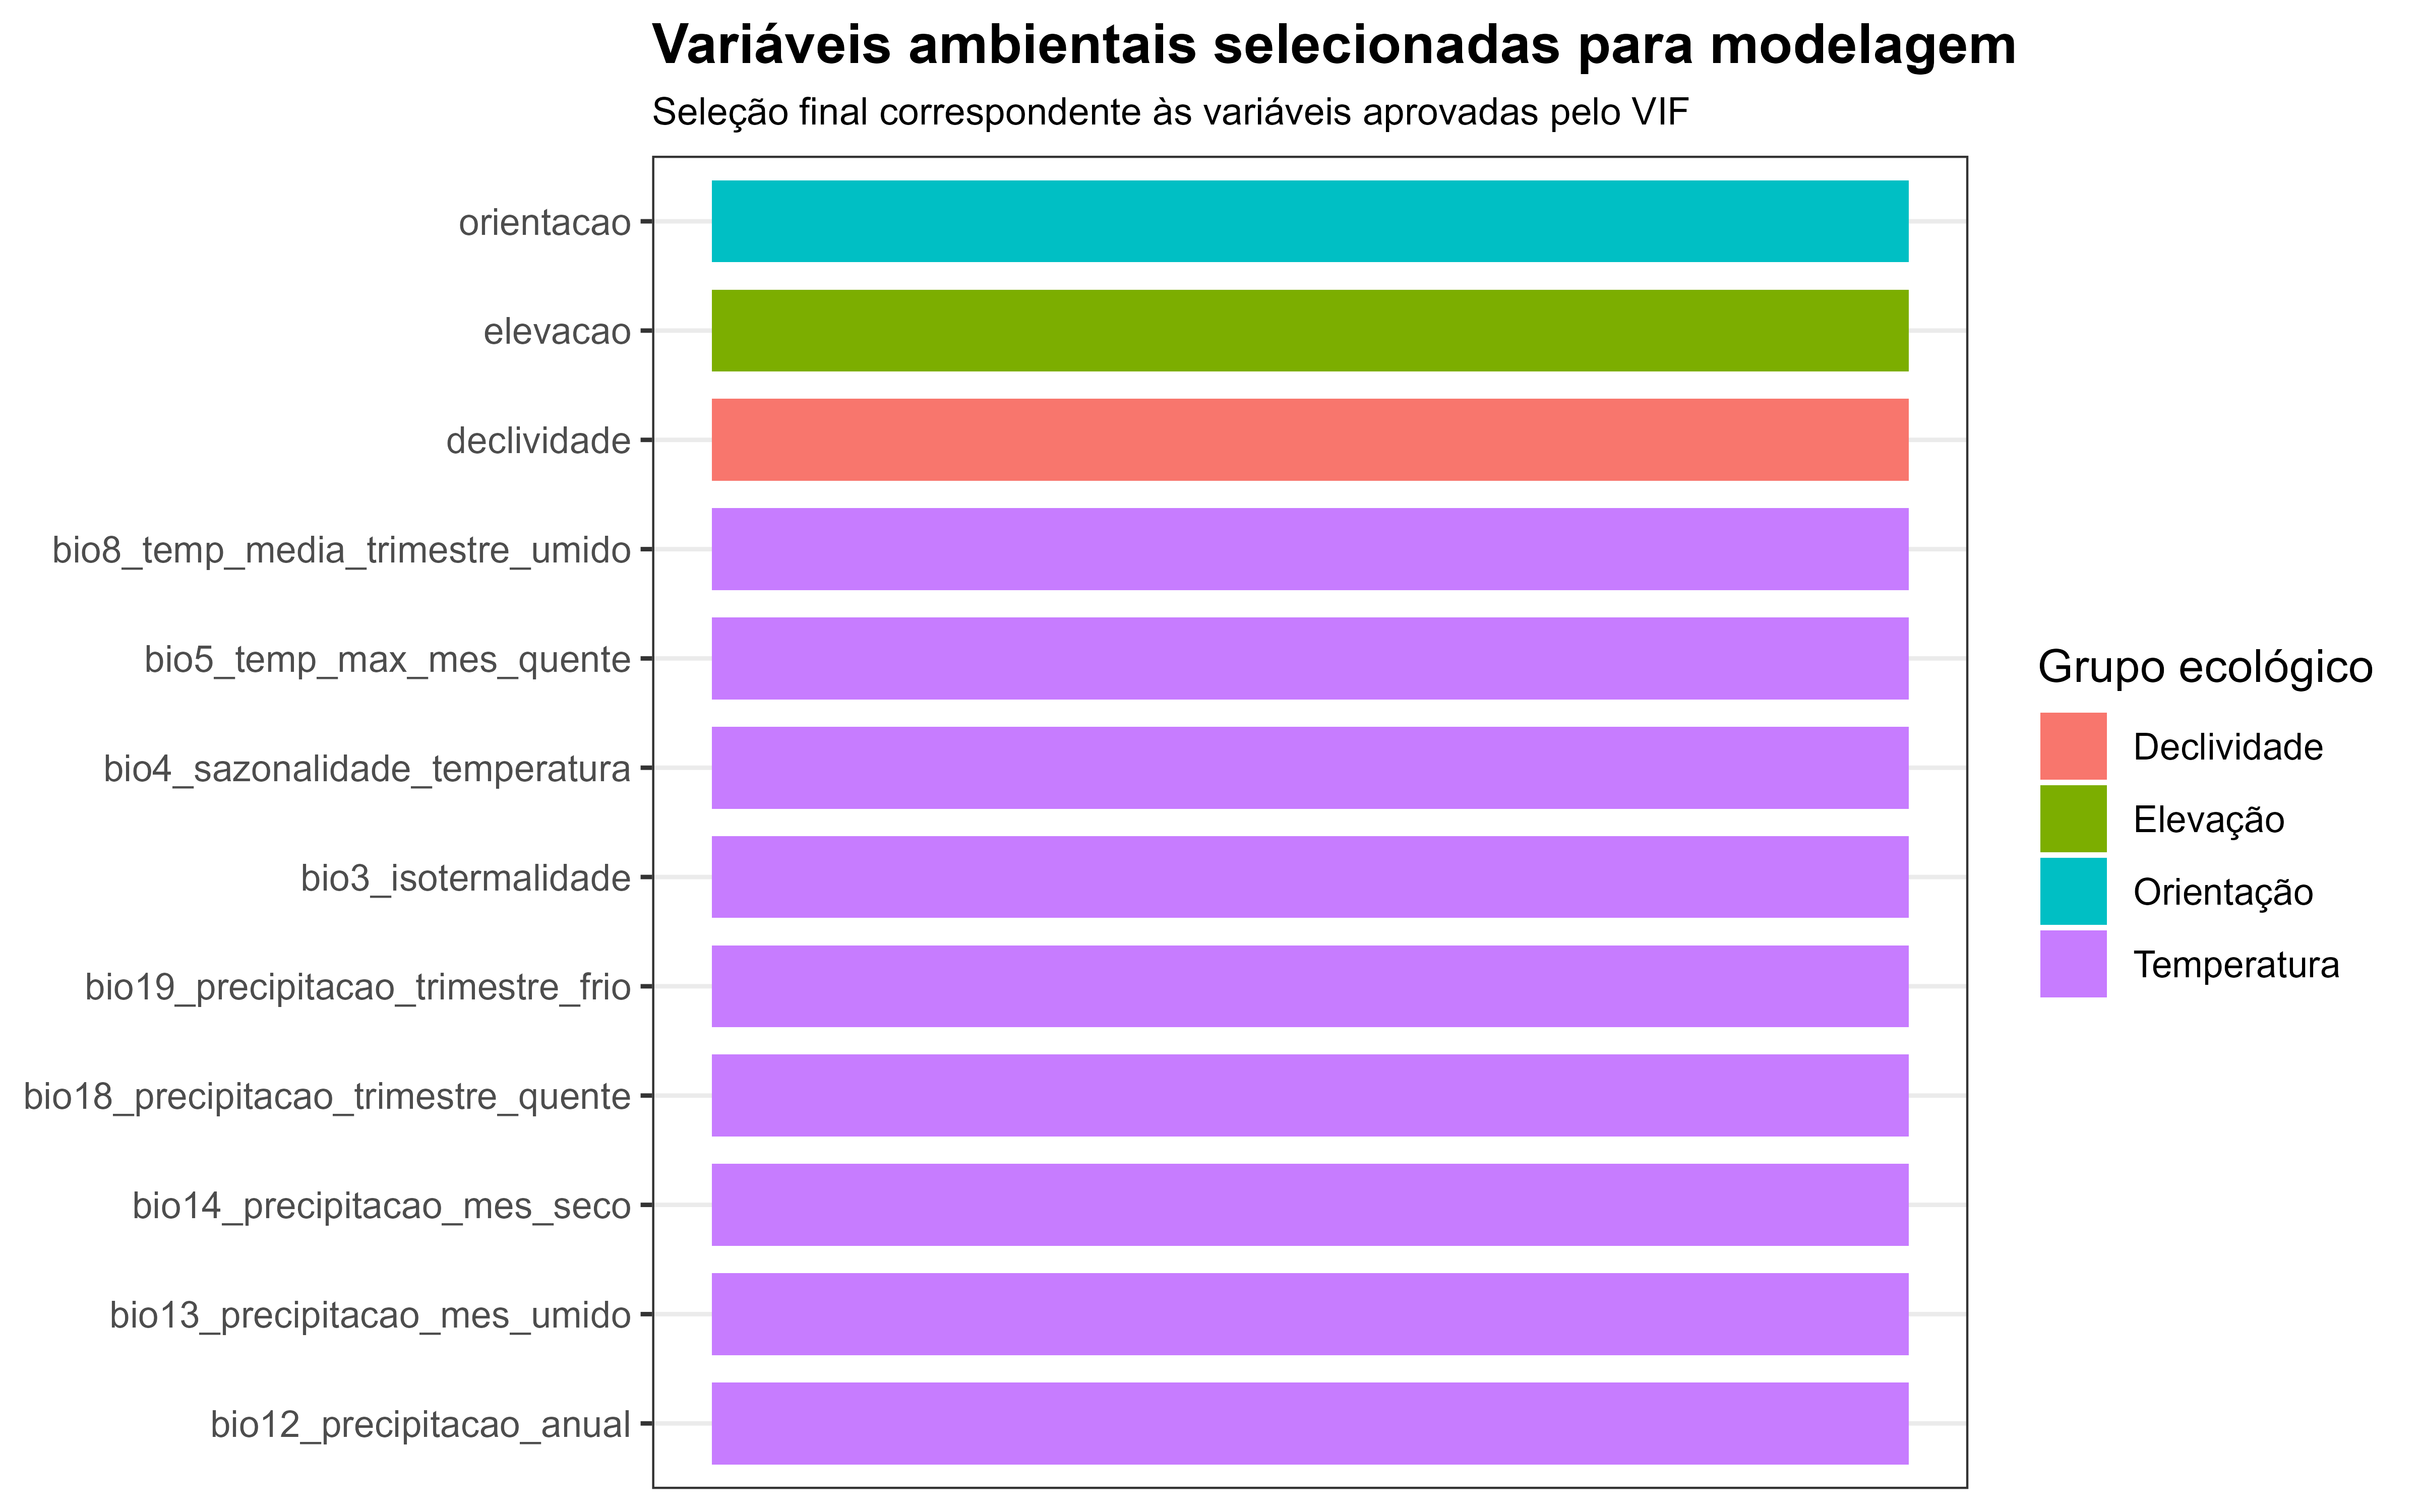
\includegraphics[width=0.85\textwidth]
	{figuras/unidade04/unidade04_variaveis_selecionadas.png}
	\caption{
		Conjunto final de variáveis ambientais selecionadas
		após análise de correlação, VIF e interpretação ecológica.
		Essas variáveis serão utilizadas nas unidades subsequentes
		para ajuste dos modelos de distribuição de espécies.
	}
	\label{fig:unidade04_variaveis_final}
\end{figure}

\section{PCA aplicada a SDM}

A Análise de Componentes Principais (PCA) é uma estratégia de redução dimensional que transforma variáveis correlacionadas em novos eixos ortogonais. Esses eixos, chamados componentes principais, são combinações lineares das variáveis originais e não são correlacionados entre si.

Em SDM, a PCA pode ser útil quando existe forte colinearidade entre variáveis ambientais e o objetivo é representar o espaço ambiental de forma compacta. Entretanto, a PCA reduz a interpretabilidade ecológica direta, pois os componentes representam combinações de variáveis, não gradientes simples como temperatura ou precipitação.

\begin{conceito}[title={\faBook\quad PCA como ortogonalização}]
	A PCA não escolhe variáveis. Ela transforma um conjunto de variáveis correlacionadas em eixos independentes. Isso reduz colinearidade, mas exige cuidado na interpretação ecológica dos componentes.
\end{conceito}

\rscriptfile{scripts/unidade04/06_pca_variaveis.R}

\begin{figure}[H]
	\centering
	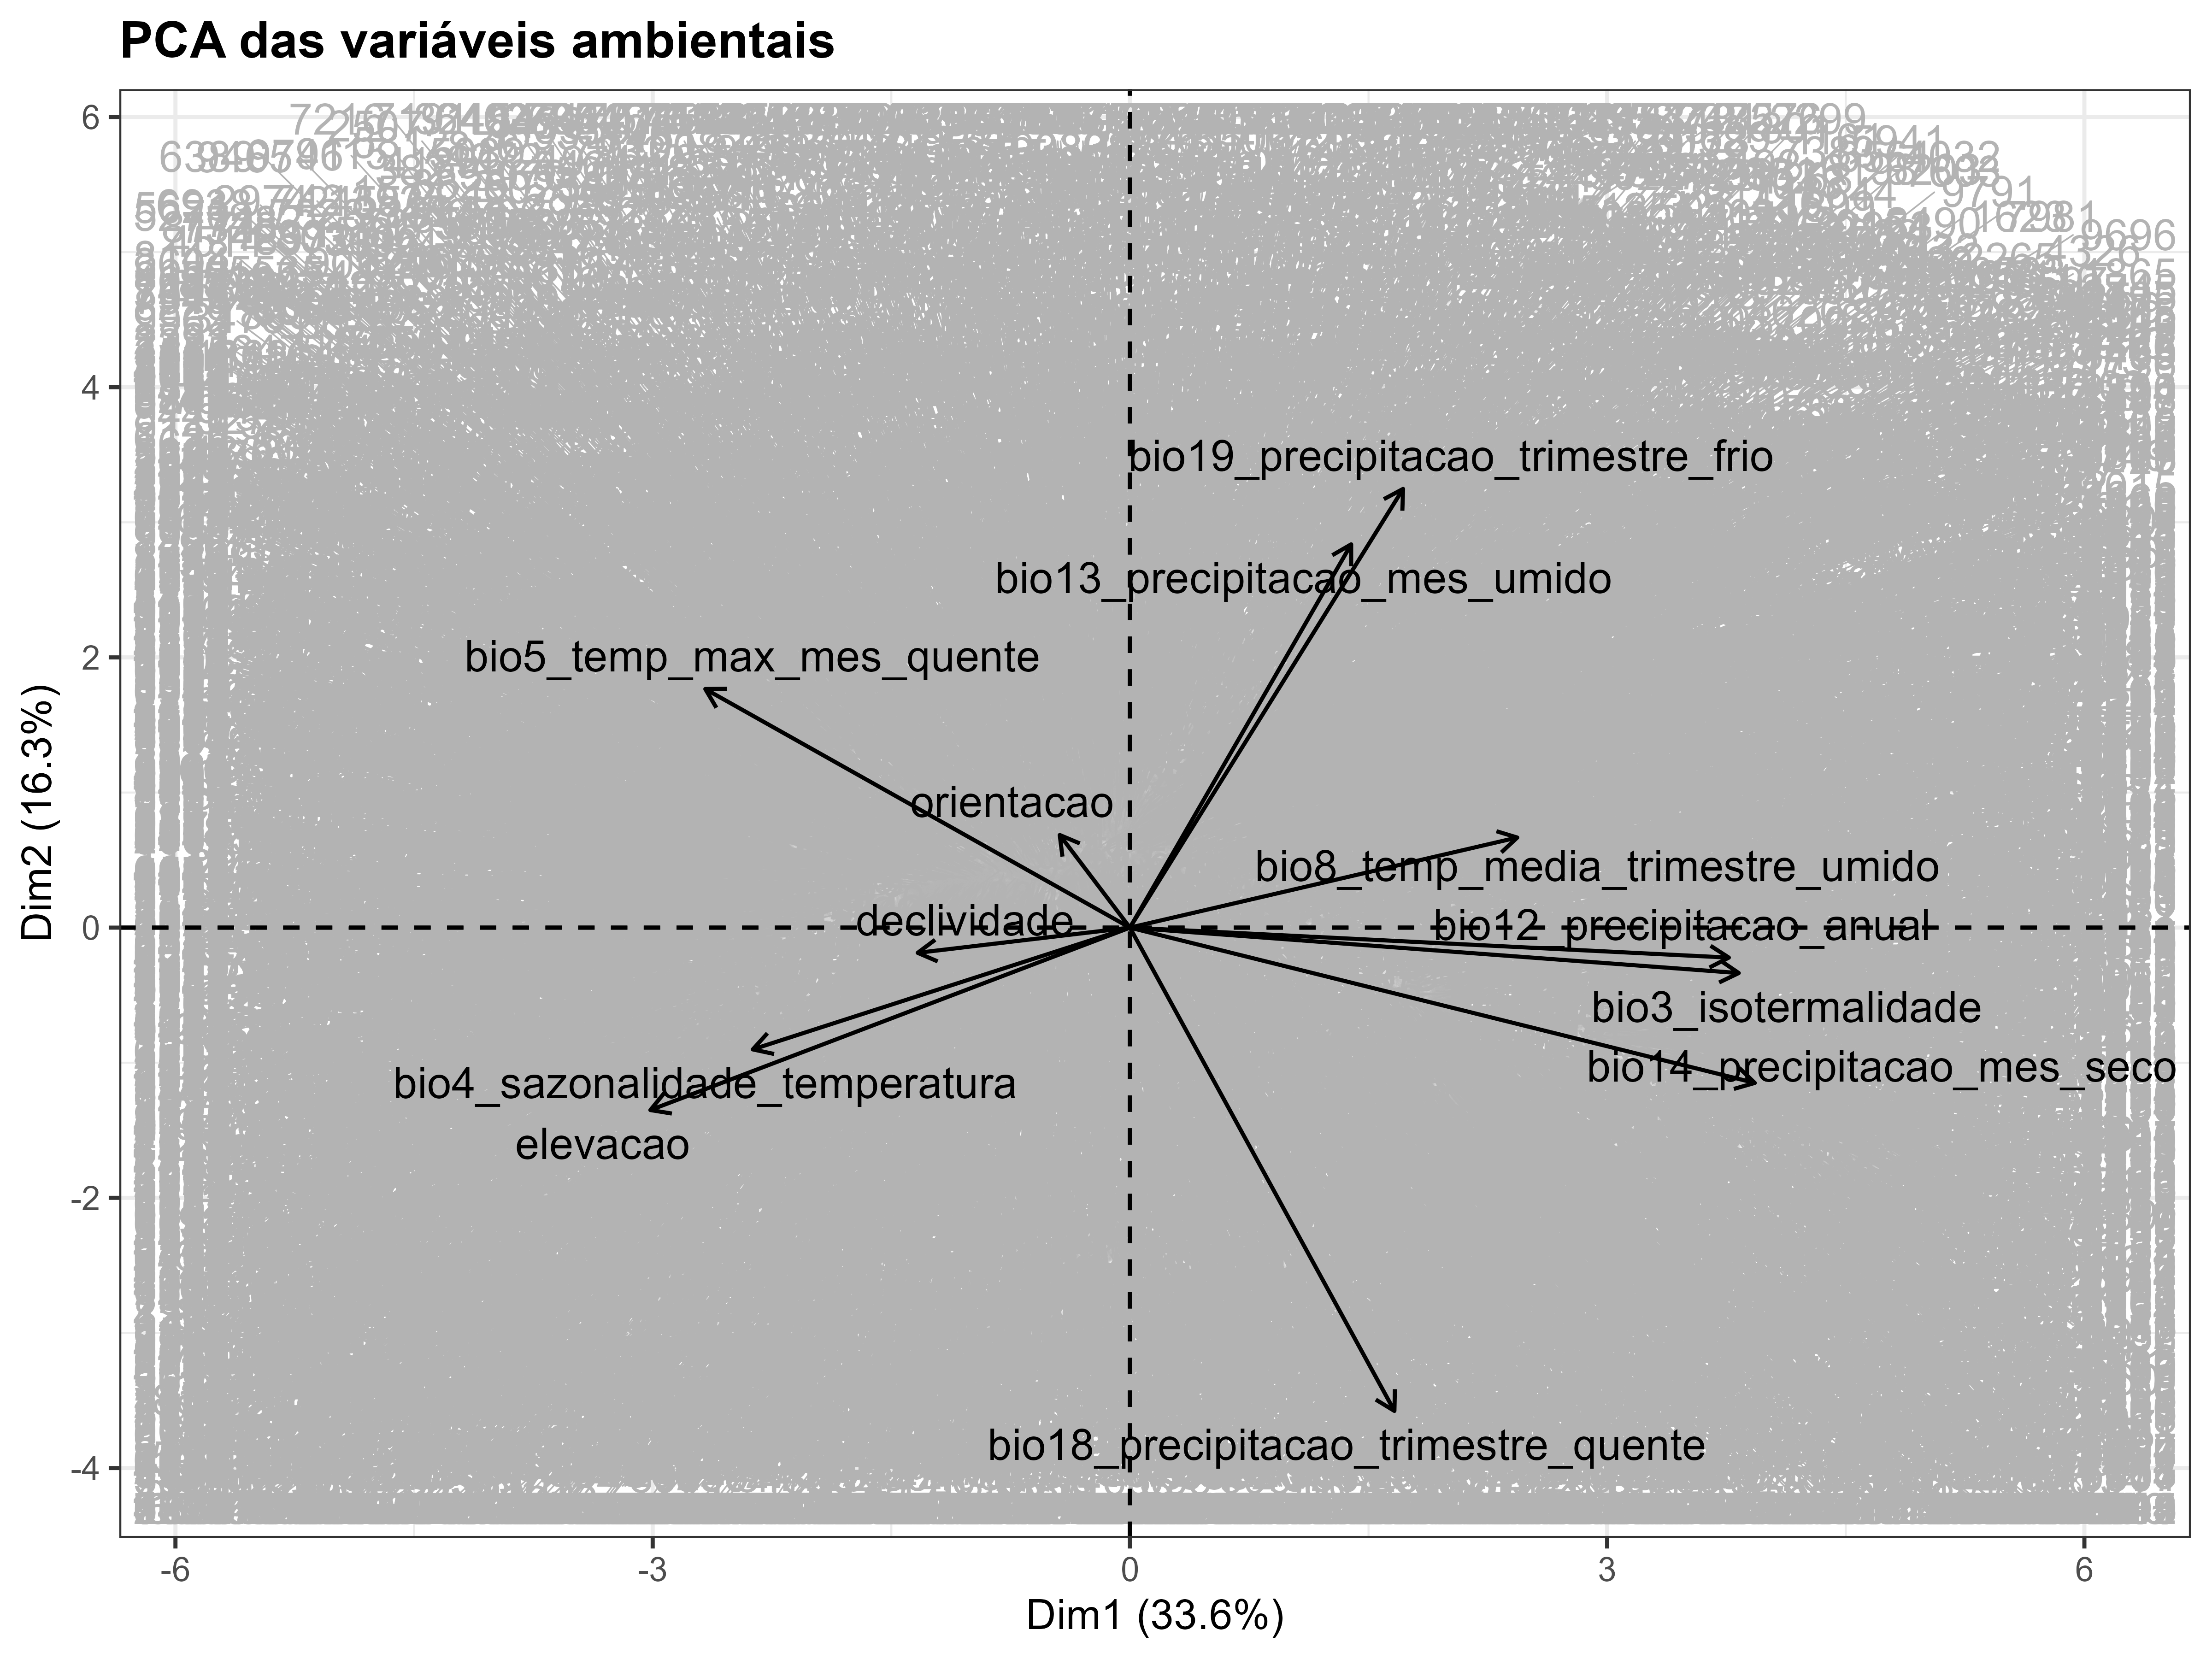
\includegraphics[width=0.90\textwidth]
	{figuras/unidade04/unidade04_pca_biplot_variaveis.png}
	\caption{
		Análise de Componentes Principais (PCA)
		das variáveis ambientais utilizadas no estudo de caso.
		Os vetores representam a contribuição de cada variável
		para os principais gradientes ambientais do bioma Amazônia.
	}
	\label{fig:unidade04_pca_biplot}
\end{figure}

\begin{figure}[H]
	\centering
	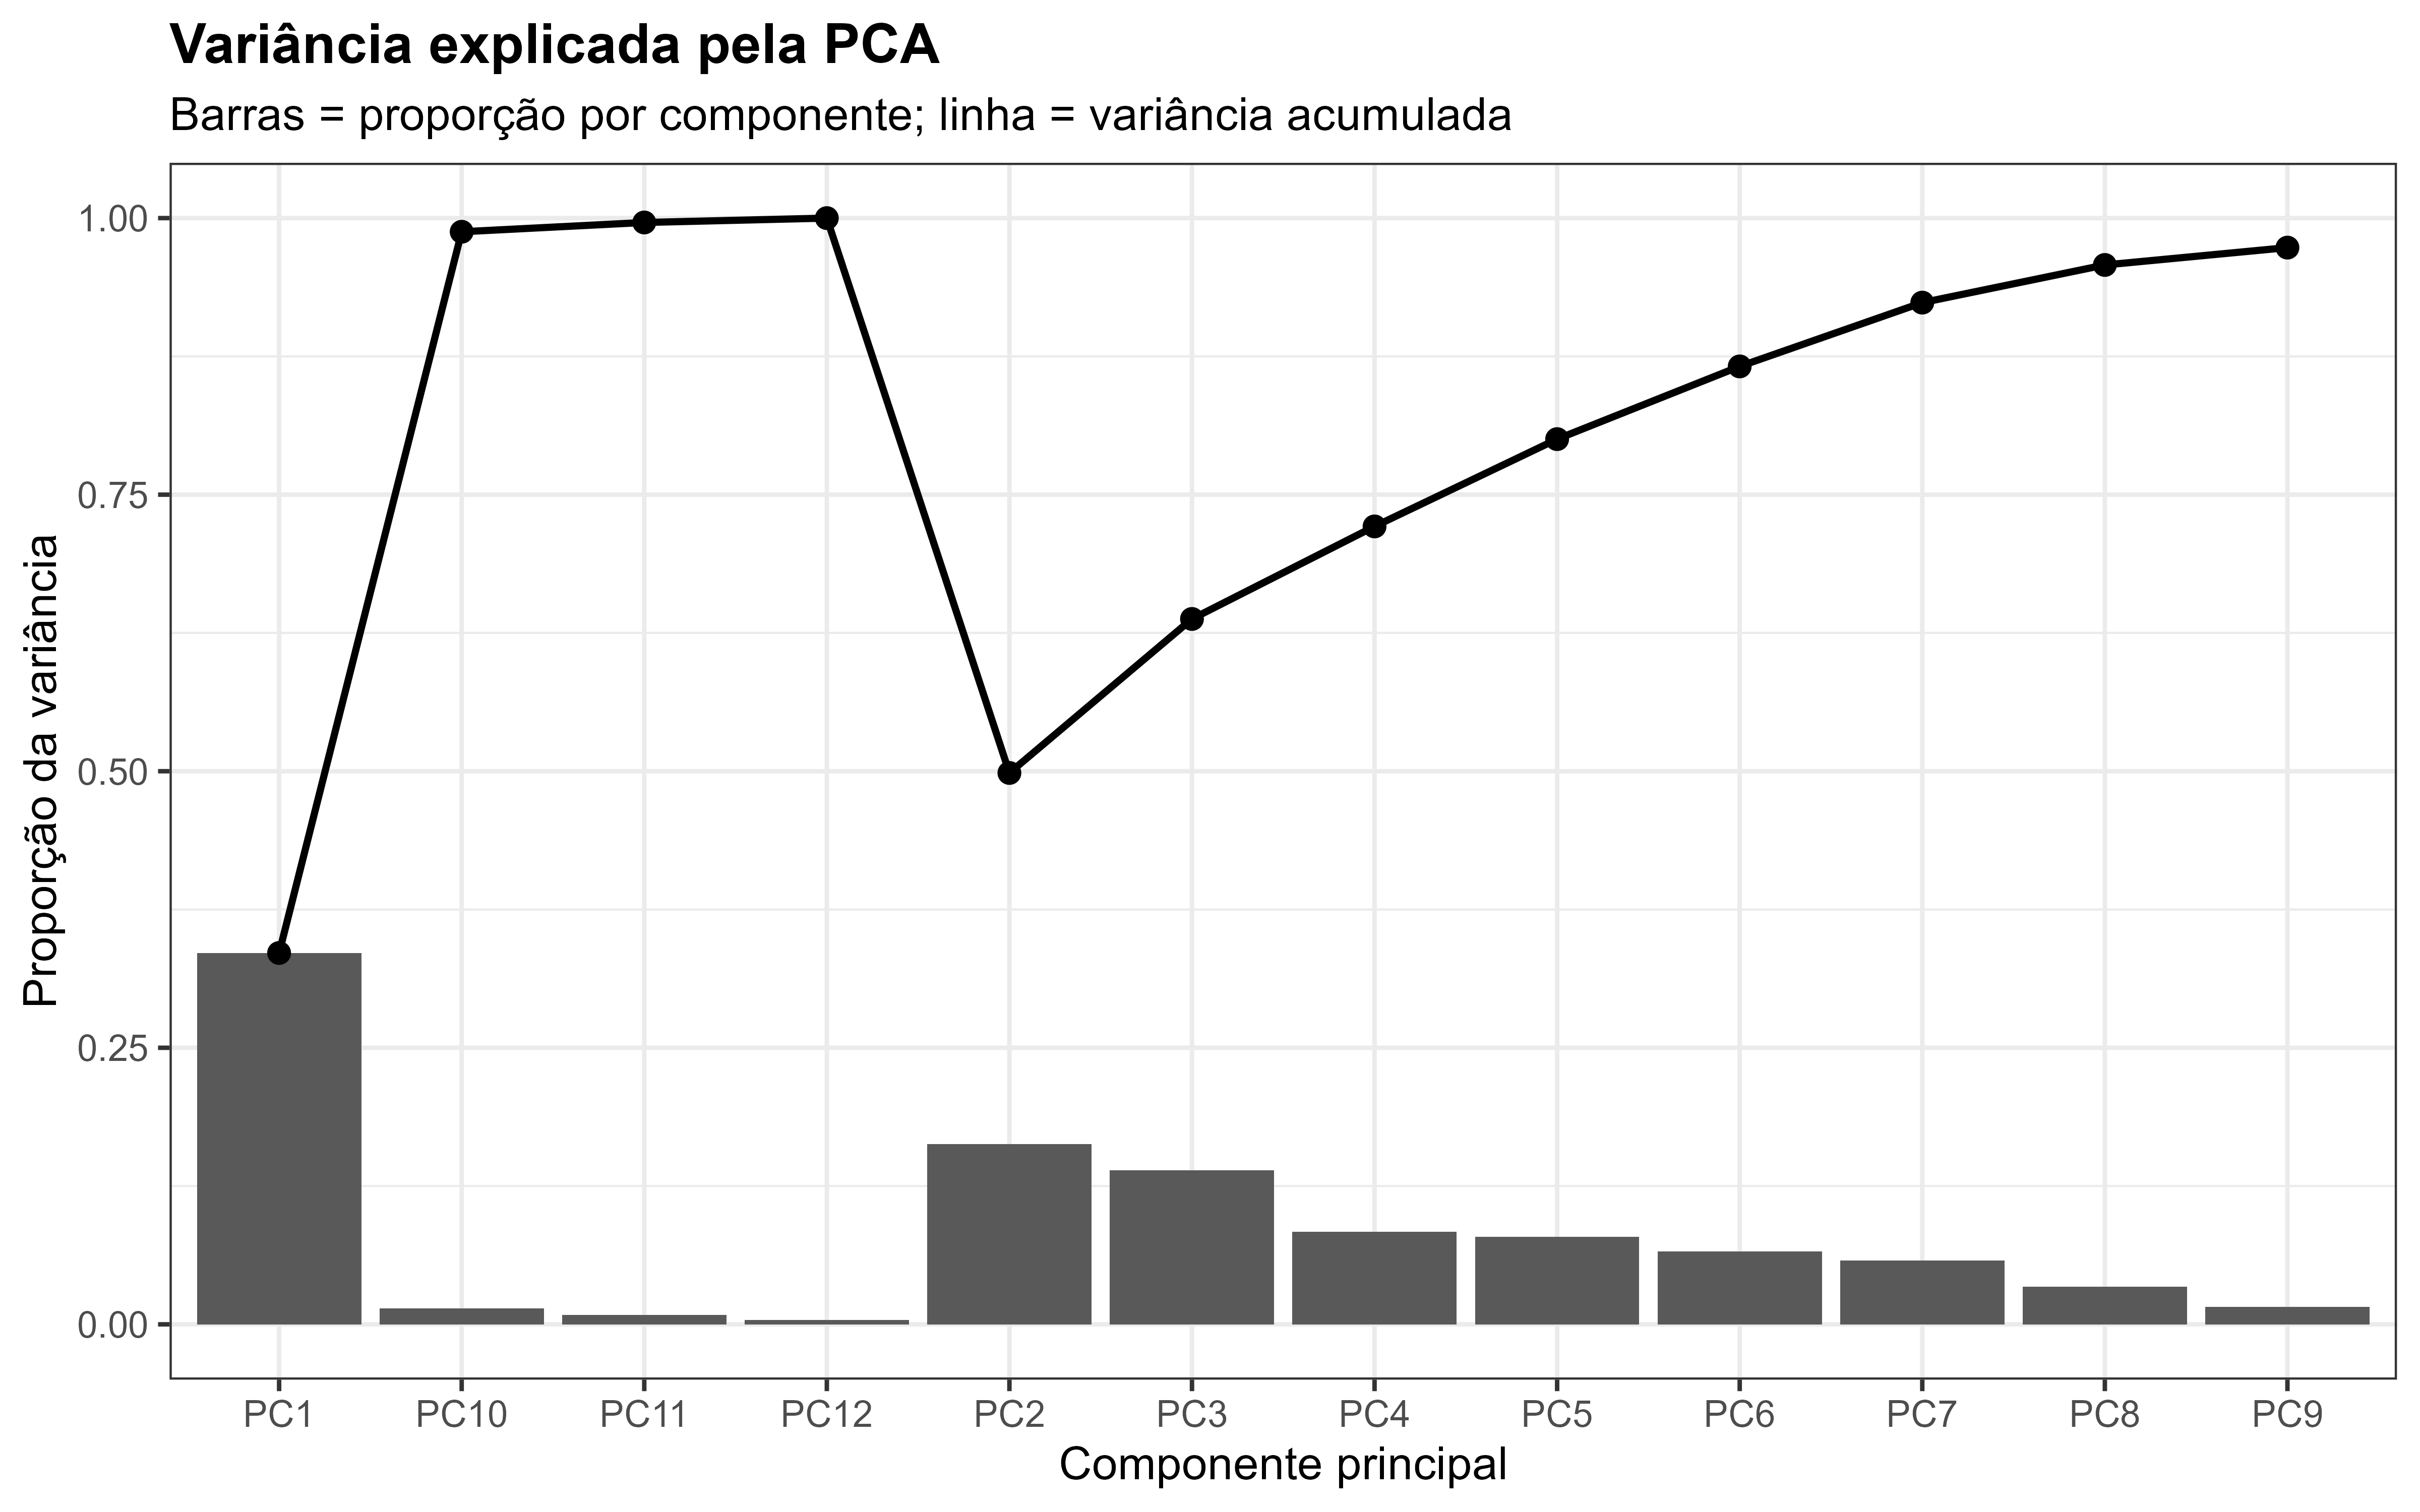
\includegraphics[width=0.80\textwidth]
	{figuras/unidade04/unidade04_pca_variancia.png}
	\caption{
		Proporção da variância explicada pelos componentes principais.
		As barras representam a contribuição individual de cada eixo,
		enquanto a linha representa a variância acumulada.
	}
	\label{fig:unidade04_pca_variancia}
\end{figure}

\begin{aplicacao}
	As Figuras~\ref{fig:unidade04_pca_biplot}
	e~\ref{fig:unidade04_pca_variancia}
	mostram que grande parte da estrutura ambiental
	do bioma Amazônia pode ser representada por poucos
	eixos ambientais principais.
	
	A PCA não substitui a seleção ecológica de variáveis,
	mas auxilia na identificação de redundâncias e na interpretação
	dos gradientes ambientais que estruturam a distribuição
	de \textit{Dinizia excelsa}.
\end{aplicacao}

\section{Pipeline integrador}

O script final reúne as etapas da Unidade 4: simulação de variáveis ambientais, análise de correlação, diagnóstico por VIF, seleção de variáveis e PCA.

\rscriptfile{scripts/unidade04/08_pipeline_multicolinearidade.R}

\section{Síntese da unidade}

A multicolinearidade é um problema central em SDM porque afeta interpretação, estabilidade e transferibilidade dos modelos. Correlação, VIF e PCA são ferramentas complementares. A correlação identifica redundância par a par; o VIF avalia redundância multivariada; e a PCA transforma variáveis correlacionadas em eixos independentes. A escolha entre remover variáveis ou usar PCA depende da pergunta científica, do algoritmo, da necessidade de interpretação ecológica e do objetivo de projeção espacial ou temporal.

\begin{conceito}[title={\faBook\quad Mensagem central da Unidade 4}]
	A seleção de variáveis não é apenas um procedimento estatístico.
	O objetivo é construir um conjunto de preditores que represente
	os principais filtros ecológicos associados à distribuição da espécie,
	evitando redundâncias excessivas e aumentando a interpretabilidade
	dos modelos.
	
	As variáveis selecionadas nesta unidade serão utilizadas
	nas Unidades 5 a 17 para modelagem, avaliação,
	projeções climáticas e aplicações à conservação.
\end{conceito}

\begin{aplicacao}
	As variáveis selecionadas nesta unidade serão utilizadas nas etapas subsequentes de modelagem. A partir deste ponto, o conjunto ambiental passa a representar uma hipótese ecológica refinada sobre os fatores que influenciam a distribuição de \textit{Dinizia excelsa} na Amazônia.
	
	Na próxima unidade, essas variáveis serão integradas à definição da área acessível (M) dentro do framework BAM.
\end{aplicacao}

\section{Exercícios de fixação}

\begin{enumerate}
	\item Explique o que é multicolinearidade e por que ela é comum em variáveis ambientais.
	\item Diferencie correlação de Pearson e correlação de Spearman.
	\item Por que duas variáveis altamente correlacionadas não devem ser mantidas automaticamente no mesmo modelo?
	\item Explique o significado do VIF.
	\item Qual é a diferença entre diagnóstico por correlação e diagnóstico por VIF?
	\item Em que situações a PCA pode ser útil em SDM?
	\item Discuta uma desvantagem ecológica de usar componentes principais como preditores.
\end{enumerate}

% ============================================================
% UNIDADE 5
% ============================================================
